\documentclass[12pt]{article}

\usepackage[top = 1in, bottom = 1in, left = 0.75in, right = 0.75in]{geometry}
\usepackage{amsmath, amssymb, amsthm}
\usepackage{graphicx}
\usepackage{float}
\usepackage{xcolor}



\theoremstyle{definition}
\newtheorem{question}{Question}
\newenvironment{answer}{
    \textbf{\textit{Answer:}} \qquad
}{\hfill $\blacksquare$ \\ \begin{center}
    \rule{0.6\linewidth}{0.5px}    
\end{center}
}


% CUSTOM DEFINITIONS
\newcommand{\R}{\mathbb{R}}
\newcommand{\Z}{\mathbb{Z}}
\newcommand{\C}{\mathbb{C}}
\newcommand{\zcal}{\mathcal{Z}}
\newcommand{\inv}[1][1]{^{(- #1)}}


\title{Solution to Time Series Assignment}
\author{Subhrajyoty Roy (MB1911)}
\date{\today}

\begin{document}
\maketitle

\begin{center}
    \rule{0.8\textwidth}{1px} 
\end{center}
\vspace*{2em}

% Q1
\begin{question}
    Write a short note explaining applications of Time Series analysis.
\end{question}

\begin{answer}
    While the time series methodologies have been used since the birth of philosophy in ancient Greece, the theoretical developments in time series analysis started early with stochastic processes much later. The first actual application of autoregressive models to data can be brought back to the work of G. U Yule and J. Walker in the 1920s and 1930s, which was later extended to ARMA model by Herman Wold. However, it took until 1970 to formalize the time series modelling, estimation, testing approaches in an organized method, by publication of the classic book ``Time Series Analysis" by G. E. P. Box and G. M. Jenkins. 

    The goal of time series analysis is primarily two-fold. The first is to provide a meaningful compact description of the available data in terms of trend, seasonal and cyclical components, and the modelling of the stochastic component using stationary autoregressive or moving average models. In engineering, signal estimation and noise removal could be classified under this goal. On the other hand, time series analysis is also heavily used for forecasting purposes across all forms of industries for prediction of future stock prices, market sales of different products (demand prediction), weather reports, and even for the prediction of future patient counts during an epidemic (e.g. covid-19) to aid the decision-making process for administrative purposes.

    Time series analysis has an enormous amount of applications in many diverse fields ranging from economics and financial modelling to engineering and science, from geology and meteorology to linguistics modelling. Any data which is recorded over successive time-periods can be subjected to time series analysis.

    \begin{enumerate}
        \item \textbf{Demography: } Time series analysis in demography dates back to 1662, by the hands of John Graunt, a 17th-century London haberdasher. His study about the mortality rates of people and creation of life tables started the field of Demography. In his analysis, he used moving average methods and a form of exponential smoothing that we use in time series analysis even today.
        \item \textbf{Medicine and Biology: } Time series analysis made its way into medicine when the first practical electrocardiograms (ECGs), which can diagnose cardiac conditions by recording the electrical signals passing through the heart, were invented in 1901. Several time series techniques to find the outliers and abnormal patterns in recorded heartbeats are used even today to detect cardiac problems of a patient.
        \item \textbf{Signal Estimation: } During world war II, time series analysis has been extensively used in signal processing by N. Wiener, R. E. Kalman, D. Gabor using harmonic analysis, spectral analysis etc. Noise removal from the distorted signal, signal reduction and reconstruction are few popular applications of time series in engineering.
        \item \textbf{Weather Forecasting: } In the 1850s, with Robert FitzRoy's appointment to the government department to record and publish weather-related data for sailors, time-series methodologies started to prove useful for weather forecasting. In the late 19th century, with hundreds of years of available atmospheric measurements was first assembled, when the telegraph allowed for fast compilations of atmospheric conditions in time series from many locations. By the turn of the 20th century, the idea of forecasting the weather with computational methods was vigorously pursued with the help of these compiled data sets. Currently, weather prediction is heavily used for daily weather forecasting, predicting paths of hurricanes and storms, temperature and climatology modelling.
        \item \textbf{Pattern Recognition: } Time series analysis has proved useful in various computational fields such as pattern recognition and image processing. Gesture recognition is another such application where the time series observations on the position of the hand (or finger) need to be interpolated to recognized certain actions or symbols.
        \item \textbf{Economics: } Forecasting GDP, economic growth, inflation and exchange rates, price of stocks and traded financial contracts are some of the popular use of time series in economics. Time series data can also help clustering similar group of economical assets or industries, to differentiate the growths of different economic sectors of a country.
        \item \textbf{Astronomy: } Astronomy has always relied heavily on plotting objects, trajectories, and measurements over time. As an example of the long history of time series data, one can consider the sunspot time series that were recorded in ancient China as early as 800 BC. The discovery of variable stars (which can be used to deduce galactic distances), the observation of transitory events such as supernovae (which enhance our understanding of how the universe changes over time), predicting the path of comets and cosmic objects and rockets are some of the most common usages of time series methodologies in Astronomy.
        \item \textbf{Linguistics and Geophysics: } Time series data on unstructured texts can provide useful insights about the evolution of different languages over centuries. Changepoint analysis, time series segmentation, dynamic time warping are few methodologies used to analyze such datasets. Geophysicists, on the other hand, collect and analyze centuries of time series data about earthquakes, volcanos and other physical properties of the earth, to understand the evolution process better.
    \end{enumerate}   
    In conclusion, time series analysis appears almost everywhere in the field of arts, science and commerce, and remained one of the integral components of statistics for long.
\end{answer}



% Q2
\begin{question}
    Consider an ARMA(1,1) model given by 
    $$
    X_t - \phi X_{(t-1)} = Z_t + \theta Z_{(t-1)}
    $$
    where $\phi = 0.1, \theta = 0.4$ and $Z_t \sim \text{IID}(0, \sigma^2)$ with $\sigma^2$ = 1.
    Draw a sample of size $40$, $X_1, X_2, \dots X_{40}$ from this.

    Calculate $\widehat{\rho}_1, \widehat{\rho}_2, \dots \widehat{\rho}_7$ from the data. 

    Hence, calculate $95\%$ confidence interval for $\rho_1$. Does it contain the model value of $\rho_1$?
\end{question}

\begin{answer}
    The mentioned ARMA(1, 1) model is given by

    \begin{equation}
        X_t = 0.1 X_{(t-1)} + Z_t + 0.4 Z_{(t-1)}
        \label{eqn:q2-1}    
    \end{equation}

    where $Z_t \sim \text{IID}(0, 1)$. In order to simulate samples from this ARMA(1, 1) process given in Eq.~\eqref{eqn:q2-1}, we need to use the stationary property of the process. We choose some arbitrary value of $X_0$ (say equal to $1$), and then obtain $X_1, X_2, \dots X_{B}$ for some large $B$, using Eq.~\eqref{eqn:q2-1}, where we simulate the IID noise $Z_t$ from the standard normal distribution. If $B$ is large enough, then by the assumption of stationarity, this process will converge to the stationary ARMA(1, 1) process governed by Eq.~\eqref{eqn:q2-1}. Also, in a linear process, two observations of a large enough lag are approximately independent of each other, in other words, for large $B$, $X_B$ and $X_0$ are approximately independent. Thus, after sampling large number of samples (say $B = 1000$), we can relabel $X_B$ as $X_0$ (which has converged to the correct distribution of the time series due to stationarity), and then use that $X_0$ to obtain samples $X_1, \dots X_{40}$ afterwards. 

    Using this process, we obtain the following samples of size $40$ as,

    \begin{center}
    \begin{tabular}{ccccc}
        -0.52544863 & 0.49058218 & 2.44282098 & 1.62111175 & -1.35311674\\
         -2.76172570 & -1.44865207 & -1.88252238 & -0.20526112 & -1.00769036 \\
        -0.66660304 & 0.99528053 & 0.52710766 & 0.77272032 & 0.18111537 \\
        0.69019163 & 1.64687928 & 0.46356077 & -0.19612178 & -0.73902929 \\
         -1.17983011 & -1.14527804 & -0.36549847 & -0.94203331 & -0.95896888 \\
         -2.75000384 & -2.84328258 & -2.25173083 & -2.01164934 & 0.03833377 \\
        1.53029127 & 0.26689518 & -0.48536917 & 1.18579833 & 2.62394263 \\
        0.28472562 & -1.48194893 & -3.44416159 & -1.00240464 & -0.80192971\\
    \end{tabular}
    \end{center}

    (The samples are given from left to right, rowwise). A plot of these samples are given below.

    \begin{figure}[H]
        \centering
        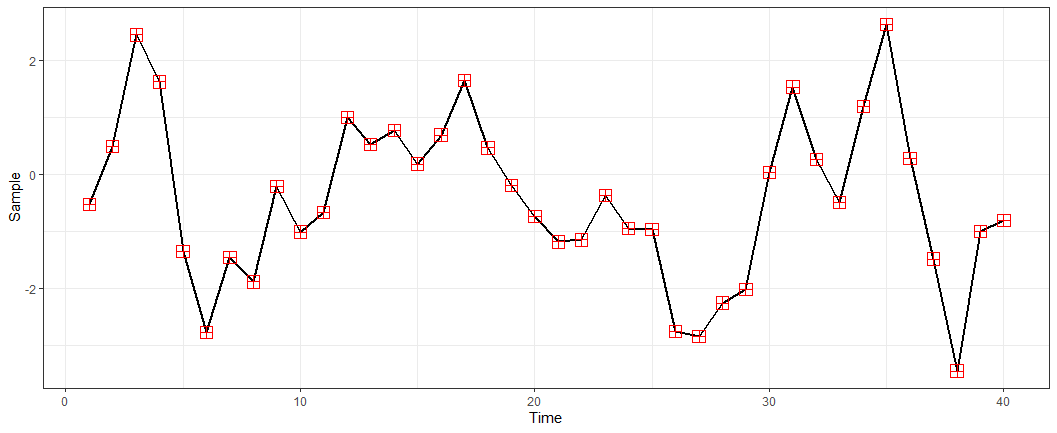
\includegraphics[width = \linewidth]{arma_samples.png}
    \end{figure}

    Now, the autocorrelation values are computed as $\widehat{\rho}(h) = \dfrac{\widehat{\gamma}(h)}{\widehat{\gamma}(0)}$, where 

    $$
    \widehat{\gamma}(h) = \dfrac{1}{40}\sum_{t = 1}^{40 - h} (x_{t+h} - \bar{x})(x_t - \bar{x})
    $$

    where $\bar{x} = \dfrac{1}{40} \sum_{t = 1}^{40} x_t$. Based on the given sample, we obtain that the sample mean $\bar{x} = -0.4172226$. Based on this, we obtain the autocovariances 
    
    \begin{multline*}
        [\widehat{\gamma}(0), \widehat{\gamma}(1), \ldots, \widehat{\gamma}(7)] \\
        = [2.0193703,  1.2025201,  0.2425296, -0.2469182, -0.2439261, -0.2354635, -0.5095807, -0.6813610]        
    \end{multline*}

    Therefore, the sample autocorrelations are given by 

    \begin{multline*}
        [\widehat{\rho}(1), \ldots \widehat{\rho}(7)]\\
        = [0.5954926,  0.1201016, -0.1222748, -0.1207932, -0.1166024, -0.2523464, -0.3374126]
    \end{multline*}


    In order to construct $95\%$ CI for $\rho(1)$, we use Bertlett's formula, which tells that $\widehat{\rho}(1) \rightarrow \mathcal{N}\left(\rho(1), w/n\right)$, where 

    \begin{align*}
        w 
        & = \sum_{l = 1}^{\infty} (\rho(l+1)\rho(l-1) - 2\rho(l)\rho(1))^2\\
        & \approx \sum_{l = 1}^{6} (\rho(l+1)\rho(l-1) - 2\rho(l)\rho(1))^2 , \qquad \text{assuming subsequent terms are small}\\
    \end{align*}

    Now, in order to estimate this $w$ from the data, we replace $\rho(h)$ by their estimate $\widehat{\rho}(h)$, for $h = 1, 2, \dots 7$ instead. This leads us to the estimate of asymptotic variance as,

    $$
    \widehat{w} = \sum_{l = 1}^{6} (\widehat{\rho}(l+1)\widehat{\rho}(l-1) - 2\widehat{\rho}(l)\widehat{\rho}(1))^2 = 0.5800527
    $$

    Therefore, the approximate $95\%$ confidence interval for $\rho(1)$ is given by,

    $$
    \left[ \widehat{\rho}(1) - 1.96\sqrt{\dfrac{\widehat{w}}{n}},
    \widehat{\rho}(1) - 1.96\sqrt{\dfrac{\widehat{w}}{n}} \right]
    = [0.359467, 0.831519]
    $$

    On the other hand, we know that the autocovariance function of ARMA(1, 1) is given as 

    $$
    \gamma(h) = \begin{cases}
        \sigma^2 \left[ 1 + \dfrac{(\theta + \phi)^2}{(1 - \phi^2)} \right] & h = 0\\
        \sigma^2 \left[ (\theta + \phi) + \dfrac{(\theta + \phi)^2\phi }{(1 - \phi^2)} \right] & h = 1\\
        \phi^{|h| - 1} \gamma(1)
    \end{cases}
    $$
    
    Hence, the true value of $\rho(1)$ for the given value $\theta = 0.4$ and $\phi = 0.1$, we have 
    
    \begin{align*}
        \rho(1) = \dfrac{\gamma(1)}{\gamma(0)} & = \left[ (\theta + \phi) + \dfrac{(\theta + \phi)^2\phi }{(1 - \phi^2)} \right] / \left[ 1 + \dfrac{(\theta + \phi)^2}{(1 - \phi^2)} \right] \\
        & = \dfrac{(\theta + \phi)(1 + \phi\theta)}{(1 + 2\theta\phi + \theta^2)} \\
        & = \dfrac{(0.4 + 0.1)(1 + 0.4 \times 0.1)}{(1 + 2\times 0.1 \times 0.4 + 0.4^2)} = 0.4193548
    \end{align*}

    The $95\%$ confidence interval for $\rho(1)$ given by $[0.359467, 0.831519]$ contains the model value $0.4193548$.
\end{answer}




% Q3
\begin{question}
    Draw random numbers $x_1, x_2, \dots x_{40}$ with $0 \leq x_i \leq 9$. Consider it as an $\text{IID}(0, \sigma^2)$ sequence. Calculate $\widehat{\rho}_1, \widehat{\rho}_2, \dots \widehat{\rho}_7$ based on this.

    On the basis of these, test for independent and identical distribution of the given sequence. (Use all $4$ methods discussed). Also, use the test based on ranks.
\end{question}

\begin{answer}
    In order to draw random numbers $x_1, x_2, \dots x_{40}$ with $0 \leq x_i \leq 9$, we use \texttt{sample} function in \texttt{R} programming language. This draws a random number between $0$ to $9$, each with equal probability of being chosen (i.e. equal to $0.1$). We draw $40$ such random numbers with repeatation. The obtained sample turns out to be as follows (samples are from left to right, rowwise),

    \begin{center}
        \begin{tabular}{cccccccccc}
            2 & 8 & 2 & 8 & 6 & 7 & 4 & 3 & 6 & 0\\
            0 & 4 & 4 & 1 & 7 & 2 & 2 & 8 & 4 & 7 \\
            1 & 9 & 4 & 7 & 4 & 7 & 0 & 2 & 2 & 2 \\
            6 & 4 & 3 & 1 & 1 & 9 & 0 & 6 & 5 & 1
        \end{tabular}
    \end{center}

    The following plot shows the generated samples as a function of time.

    \begin{figure}[H]
        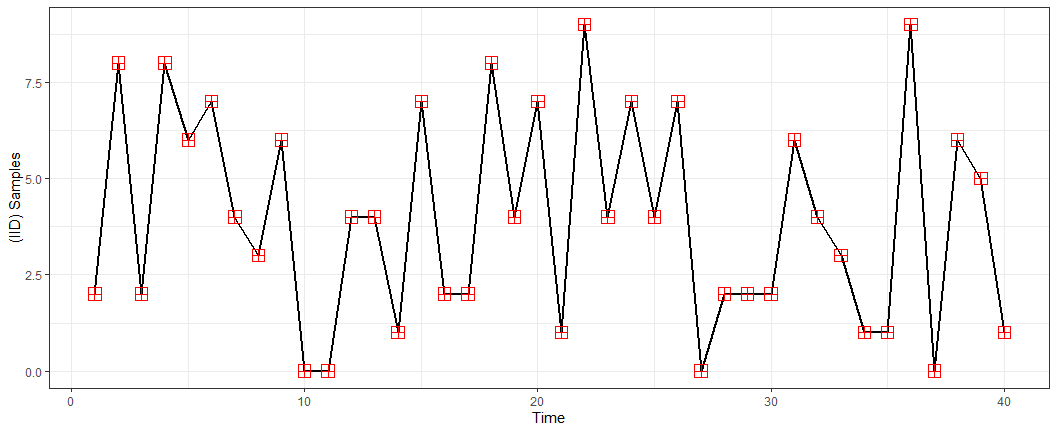
\includegraphics[width = \linewidth]{iid_seq.png}
    \end{figure}

    We use the formula mentioned above (in the answer of question 2), to find the sample autocorrelation values. Note that the sample mean turns out to be $\bar{x} = 3.975$. Next, we compute the autocovariances, 

    \begin{multline*}
        [\widehat{\gamma}(0), \ldots, \widehat{\gamma}(7)] \\
        = [7.4743750, -1.9725156,  1.5993438,  0.1243281, -0.2506875, -0.5550781, -0.3050938, 0.3717656]            
    \end{multline*}

    and hence the autocorrelations $\widehat{\rho}(h) = \dfrac{\widehat{\gamma}(h)}{\widehat{\gamma}(0)}$ turns out to be

    \begin{multline*}
        [\widehat{\rho}(1), \ldots, \widehat{\rho}(7)]\\
        = [-0.26390375,  0.21397692,  0.01663392, -0.03353959, -0.07426415, -0.04081863, 0.04973869]
    \end{multline*}

    Now, we perform testing the null hypothesis that the sampled sequence is $\text{IID}(0, \sigma^2)$ using different testing methods.
    \begin{enumerate}
        \item \textbf{Wald-type Asymptotic test:} Using the asymptotic normality of the sample autocorrelations of an iid sequence, we note that if the sequence is iid, then at $5\%$ level of significance, $95\%$ of the sample autocorrelation functions should fall between $\pm \dfrac{1.96}{\sqrt{n}} = \pm \dfrac{1.96}{\sqrt{40}} = \pm 0.3099$. We see that all of the autocorrelation values falls within this bound, hence the sample does not show sufficient evidence to reject the iid hypothesis at $5\%$ level of significance.
        \item \textbf{Simple portmanteau test:} According to this test method, the statistic $Q = n \sum_{j = 1}^h \widehat{\rho}(j)^2$ should follow asymptotically a chi-square distribution with $h$ degrees of freedom. Here with $n  = 40$ and $h = 7$, the $Q$ turns out to be $Q = 5.059527$, while the cut-off from chi-square distribution turns out to be $\chi^2_{0.95, 7} = 14.06714$ at $5\%$ level of significance. Clearly, the observed value of $Q$ is lower than the cutoff, hence the data does not show sufficient evidence to reject the null hypothesis that the sequence is $\text{IID}(0, \sigma^2)$.
        \item \textbf{Ljung and Box's test:} Here, the test statistic is $Q_{LB} = n(n+2) \sum_{j = 1}^h \dfrac{\widehat{\rho}(j)^2}{(n - j)}$. This also follows approximately a chi-square distribution with $h$ degrees of freedom. With $n = 40$ and $h = 7$, for the obtained samples this turns out to be $Q_{LB} = 5.562389$. Clearly, this observed $Q_{LB}$ is also less than the cutoff value $\chi^2_{0.95, 7} = 14.06714$ at $5\%$ level of significance. Therefore, according to this test, the data does not show sufficient evidence to reject the iid hypothesis.
        \item \textbf{Mcleod and Li's test:} The test statistic proposed by Mcleod and Li is similar to Ljung and Box, $Q_{ML} = = n(n+2) \sum_{j = 1}^h \dfrac{\widehat{\rho}_{WW}(j)^2}{(n - j)}$, where $\widehat{\rho}_{WW}(j)$ is the autocorrelations of the squared data $x_1^2, x_2^2, \dots x_{40}^2$. This statistic is again approximately distributed as a chi-squared distribution with $h$ degrees of freedom under the null hypothesis of iid sequence. Based on this squared data, the sample autocorrelation turns out to be,
        
        \begin{multline*}
            [\widehat{\rho}_{WW}(1), \widehat{\rho}_{WW}(2), \ldots, \widehat{\rho}_{WW}(7)] =
            [-0.32673257,  0.30920941, -0.07891111, \\
             0.07383917, -0.04986157, -0.09269475, -0.01291182]
        \end{multline*}

        Based on this, we have $Q_{ML} = 9.915190$, which is still less than the cutoff $\chi^2_{0.95, 7} = 14.06714$ at $5\%$ level of significance. Thus, the data again does not show any sufficient evidence to reject the iid hypothesis.

        \item \textbf{Rank test:} Rank test is useful to detecting any linear trend present in the data. Let, $P$ denotes the number of concordant pair in the dataset, i.e. the number of pairs $(x_i, x_j)$ such that $x_i < x_j$ and $i < j$. Under the assumption of null hypothesis that the data is $\text{IID}(0, \sigma^2)$, $P$ is approximately $N(\mu_p, \sigma_p^2)$ where $\mu_p = n(n-1)/4$ and $\sigma_p^2 = n(n-1)(2n + 5)/72$. Therefore, we reject the null hypothesis at $5\%$ level of significance if $|P-\mu_p| / \sigma_p > 1.96$. 
        
        For the obtained samples, we have $P = 307$, and hence $\vert P - \mu_p \vert / \sigma_p = 1.934$, which is less than the cutoff $z_{0.975} = 1.96$. Therefore, again the obtained sample does not show any sufficient evidence to reject the null hypothesis that the sample is $\text{IID}(0, \sigma^2)$.
    \end{enumerate}
\end{answer}






\end{document}
